\documentclass[12pt]{article}

\usepackage{graphicx}
\usepackage{paralist}
\usepackage{amsfonts}
\usepackage{amsmath}
\usepackage{hhline}
\usepackage{booktabs}
\usepackage{multirow}
\usepackage{multicol}
\usepackage{url}
\usepackage{hyperref}

\oddsidemargin -10mm
\evensidemargin -10mm
\textwidth 160mm
\textheight 200mm
\renewcommand\baselinestretch{1.0}

\pagestyle {plain}
\pagenumbering{arabic}

\newcounter{stepnum}

%% Comments

\usepackage{color}

\newif\ifcomments\commentstrue

\ifcomments
\newcommand{\authornote}[3]{\textcolor{#1}{[#3 ---#2]}}
\newcommand{\todo}[1]{\textcolor{red}{[TODO: #1]}}
\else
\newcommand{\authornote}[3]{}
\newcommand{\todo}[1]{}
\fi

\newcommand{\wss}[1]{\authornote{blue}{SS}{#1}}

\title{Assignment 4 Specification}
\author{Alan Scott}

%%%%%%%%%%%%%%%%Board%%%%%%%%%%%%%%%%%%%
\begin{document}

\maketitle
\newpage

\section*{Design Introduction}
\subsection*{Likely Changes}
This project was designed with the idea that the whole game of 2048 could be completely replaced with another game using a similar setup. For this reason, the 4x4 grid and the operations to carry out a game of 2048 are completely separate. The 4x4 board is defined as its own object, with only basic methods such as getters and setters for the grid data and score available. The setup for the game 2048 is a child class of Board, and it contains all the operations necessary for a 4x4 game of 2048. If you were however to create a different score based game based on a similar board, it could be re-purposed to be used for that setup.
\subsection*{Design Overview}
The design for the 2048 game involves four separate modules. The first module is Board, which emulates a 4x4 grid of numbers, and keeps track of the score. The 4x4 grid data is stored using a two dimensional array, where the rows and column of the array correspond to the rows and columns of the 2048 board. The second module, ActiveBoard, is a Board object which contains all the necessary operations inherent to the 2048 game. It is a child class of Board, and thus inherits its data structure and state variables. The third module is the GUI module, which is a specialized JFrame (ie it inherits JFrame). This module covers the graphical display of the game state, namely the 4x4 grid and the current user score. It also handles user key inputs through the implementation of the KeyListener interface. The final module of the program is Game, which is the controller that operates the various classes. It takes in user input and computes the game states through operations performed on the ActiveBoard class. When Game reaches an end state (by lack of moves or user exit) it terminates the program. 

\newpage

\subsection*{Program UML Diagram}
\begin{center}
    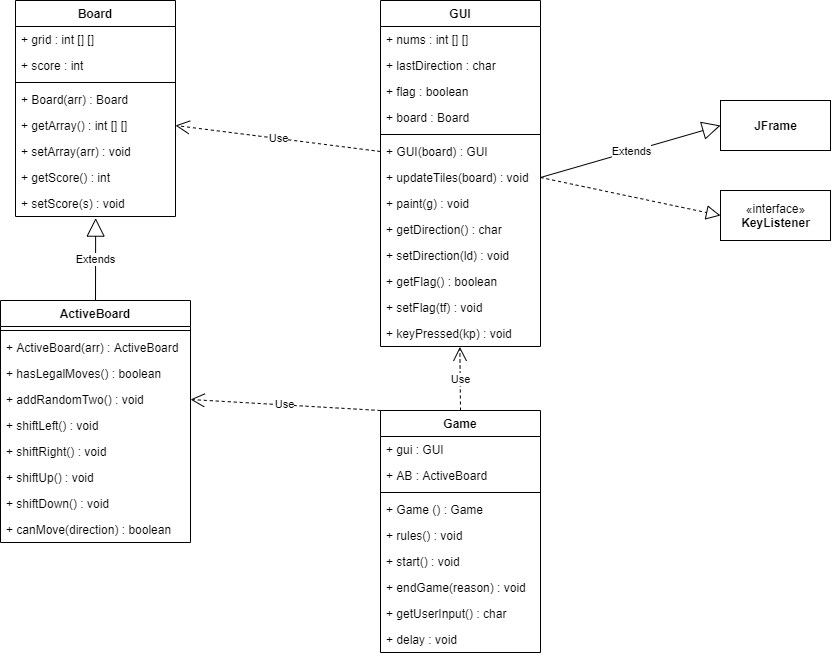
\includegraphics[scale=0.5]{A4UML.png}
\end{center}


\newpage

\section* {Board Abstract Data Type}

\subsection*{Module}

Board

\subsection* {Uses}

None

\subsection* {Syntax}

\subsubsection* {Exported Constants}

None

\subsubsection* {Exported Types}

None

\subsubsection* {Exported Access Programs}

\begin{tabular}{| l | l | l | p{5cm} |}
\hline
\textbf{Routine name} & \textbf{In} & \textbf{Out} & \textbf{Exceptions}\\
\hline
new Board & sequence[4] of sequence[4] of $\mathbb{N}$ & Board & \\
\hline
getArray & & sequence[4] of sequence[4] of $\mathbb{N}$ & ~\\
\hline
setArray & sequence[4] of sequence[4] of $\mathbb{N}$ & & ~\\
\hline
getScore & & $\mathbb{N}$ &~\\
\hline 
setScore & $\mathbb{N}$ & & ~\\
\hline
hasZero & & $\mathbb{B}$ &~\\
\hline
\end{tabular}

\subsection* {Semantics}

\subsubsection* {State Variables}

$\mathit{grid}: \text{sequence[4] of sequence[4] of } \mathbb{N}$\\
$\mathit{score}: \mathbb{N}$

\subsubsection* {State Invariant}

None

\subsubsection* {Assumptions}

Assuming the input size of the 2D array will always be 4x4

\subsubsection*{Design Decision}

The grid of the 2048 board was chosen to be represented as a 2D array of size 4x4, with the dimensions of the array corresponding to the dimensions of the 2048 board. The coordinates of the board are as follows:
\begin{table}[h]
\centering
\begin{tabular}{|l|l|l|l|}
\hline
(0,0) &  &  & (0,4) \\ \hline
      &  &  &       \\ \hline
      &  &  &       \\ \hline
(4,0) &  &  & (4,4) \\ \hline
\end{tabular}
\end{table}

\subsubsection* {Access Routine Semantics}

\noindent new Board($\mathit{arr}$):
\begin{itemize}
\item transition: $\mathit{grid} := \mathit{arr}$
\item output: $out := \mbox{self}$
\item exception: none
\end{itemize}

\noindent getArray():
\begin{itemize}
\item transition: none
\item output: $\mathit{out} := \mathit{grid}$
\item exception: none
\end{itemize}

\noindent setArray($\mathit{arr}$):
\begin{itemize}
\item transition: $\mathit{grid} := \mathit{arr}$
\item output: none
\item exception: none
\end{itemize}

\noindent getScore():
\begin{itemize}
\item transition: none
\item output: $\mathit{out} := \mathit{score}$
\item exception: none
\end{itemize}

\noindent setScore($\mathit{s}$):
\begin{itemize}
\item transition: $\mathit{grid} := \mathit{s}$
\item output: none
\item exception: none
\end{itemize}

\noindent hasZero():
\begin{itemize}
\item transition: none
\item output: $\mathit{out} := (0 \in grid)$
\item exception: none
\end{itemize}

\newpage

%%%%%%%%%%%%ActiveBoard%%%%%%%%%%%%%%%%%%%

\section* {Board Operations Module}

\subsection*{Module}

ActiveBoard

\subsection* {Uses}

Board

\subsection* {Syntax}

\subsubsection* {Exported Constants}

None

\subsubsection* {Exported Types}

None

\subsubsection* {Exported Access Programs}

\begin{tabular}{| l | l | l | p{5cm} |}
\hline
\textbf{Routine name} & \textbf{In} & \textbf{Out} & \textbf{Exceptions}\\
\hline
new ActiveBoard & sequence[4] of sequence[4] $\mathbb{N}$ & ActiveBoard &~\\
\hline
hasLegalMoves & & $\mathbb{B}$ &~\\
\hline
addRandomTwo & & &~\\
\hline
shiftLeft & & &~\\
\hline
shiftRight & & &~\\
\hline
shiftUp & & &~\\
\hline
shiftDown & & &~\\
\hline
canMove & char & $\mathbb{B}$ &~\\
\hline
\end{tabular}

\subsection*{Semantics}

\subsubsection*{State Variables}

$\mathit{grid}: \text{sequence[4] of sequence[4] of } \mathbb{N}$\\
$\mathit{score}: \mathbb{N}$ \\
\# Both of these state variables are inherited from Board

\subsubsection*{State Invariant}

None

\subsubsection*{Assumptions}

Assuming the array input to the constructor will be of size 4x4.

\subsubsection*{Access Routine Semantics}

\noindent new ActiveBoard(arr)
\begin{itemize}
    \item transition: score = 0, grid = arr
    \item output: $out := self$
    \item exception: none
\end{itemize}

\noindent hasLegalMoves()
\begin{itemize}
    \item transition: none
    \item output: $out := (0 \in grid \implies True| \exists i,j | grid[i][j] = grid[i+1][j] \implies True | grid[i][j] = grid[i][j+1] \implies True| True \implies False)$ \\
    \# if a given 2D grid contains a zero or two adjacent identical values, the it is possible for a legal move to be made.
    \item exception: none
\end{itemize}

\noindent addRandomTwo()
\begin{itemize}
    \item transition: $(\exists i,j | 0 \leq i \leq 3,0 \leq j \leq 3 | grid[i][j] = 0) \land grid[i][j] = (randInt() < 0.9 \implies 2 | True \implies 4)$ \\
    \# choose a random element $grid[i][j]$ which equals zero and set it to 2, with a 10\% chance of setting it to 4.
    \item output: none
    \item exception: none
\end{itemize}

\noindent shiftLeft()
\begin{itemize}
    \item transition: $grid := (\exists n | n > j|grid[i][j] = grid[i][n] \implies grid[i][j] = grid[i][j]+grid[i][n]) \land grid[i][n] = 0) \land (\exists m | m > j| grid[i][j] = 0 \land grid[i][m] \neq 0 \implies grid[i][j],grid[i][m] = grid[i][m],grid[i][j])$ \\
    \# If two horizontally adjacent items (or items separated by a 0) are the same value, sum them in the leftmost element, and make the rightmost element blank. Then, shift all of the elements to the left.
    \item output: none
    \item exception: none
\end{itemize}

\noindent shiftRight()
\begin{itemize}
    \item transition: $grid := (\exists n | n < j|grid[i][j] = grid[i][n] \implies grid[i][j] = grid[i][j]+grid[i][n]) \land grid[i][n] = 0) \land (\exists m | m < j| grid[i][j] = 0 \land grid[i][m] \neq 0 \implies grid[i][j],grid[i][m] = grid[i][m],grid[i][j])$ \\
    \# If two horizontally adjacent items (or items separated by a 0) are the same value, sum them in the rightmost element, and make the leftmost element blank. Then, shift all of the elements to the right.
    \item output: none
    \item exception: none
\end{itemize}

\noindent shiftUp()
\begin{itemize}
    \item transition: $grid := (\exists n | n > j|grid[i][j] = grid[n][j] \implies grid[i][j] = grid[i][j]+grid[n][j]) \land grid[n][j] = 0) \land (\exists m | m > j| grid[i][j] = 0 \land grid[m][j] \neq 0 \implies grid[i][j],grid[m][j] = grid[m][j],grid[i][j])$ \\
    \# If two vertically adjacent items (or items separated by a 0) are the same value, sum them in the uppermost element, and make the lower element blank. Then, shift all of the elements upward.
    \item output: none
    \item exception: none
\end{itemize}

\noindent shiftDown()
\begin{itemize}
    \item transition: $grid := (\exists n | n < j|grid[i][j] = grid[n][j] \implies grid[i][j] = grid[i][j]+grid[n][j]) \land grid[n][j] = 0) \land (\exists m | m < j| grid[i][j] = 0 \land grid[m][j] \neq 0 \implies grid[i][j],grid[m][j] = grid[m][j],grid[i][j])$ \\
    \# If two vertically adjacent items (or items separated by a 0) are the same value, sum them in the lowermost element, and make the upper element blank. Then, shift all of the elements downward.
    \item output: none
    \item exception: none
\end{itemize}

\noindent canMove(direction)
\begin{itemize}
    \item transition: none
    \item output: $out:= $\\
    $(direction = "D") \implies (\exists i,j| 0 \leq i,j \leq 3|(grid[i][j] = grid[i-1][j] \land grid[i][j] \neq 0) \lor (grid[i][j] = 0 \land grid[i-1] \neq 0))$ \\
    $(direction = "U") \implies (\exists i,j| 0 \leq i,j \leq 3|(grid[i][j] = grid[i+1][j] \land grid[i][j] \neq 0) \lor (grid[i][j] = 0 \land grid[i+1] \neq 0))$ \\
    $(direction = "R") \implies (\exists i,j| 0 \leq i,j \leq 3|(grid[i][j] = grid[i][j-1] \land grid[i][j] \neq 0) \lor (grid[i][j] = 0 \land grid[i][j-1] \neq 0))$ \\
    $(direction = "L") \implies (\exists i,j| 0 \leq i,j \leq 3|(grid[i][j] = grid[i][j+1] \land grid[i][j] \neq 0) \lor (grid[i][j] = 0 \land grid[i][j+1] \neq 0))$ \\
    \# given a direction ['L', 'R', 'U', 'D'] corresponding to the directions [left,right,up,down], determine if there exists a zero that can be shifted into when shifting in that direction, or if values adjacent on that shift axis are the same, and can be merged.
    \item exception: none
\end{itemize}

\newpage

%%%%%%%%%%%%Controller%%%%%%%%%%%%%%%%%%%%
\section* {Controller Module}

\subsection*{Module}

Game

\subsection* {Uses}

Board, ActiveBoard, GUI, JFrame, KeyListener

\subsection* {Syntax}

\subsubsection* {Exported Constants}

None

\subsubsection* {Exported Types}

None

\subsubsection* {Exported Access Programs}

\begin{tabular}{| l | l | l | p{5cm} |}
\hline
\textbf{Routine name} & \textbf{In} & \textbf{Out} & \textbf{Exceptions}\\
\hline
new Game & & Game & ~\\
\hline
\end{tabular}

\subsection* {Semantics}

\subsubsection* {State Variables}

$\mathit{gui}: GUI$\\
$\mathit{AB}: ActiveBoard$

\subsubsection*{Environment Variables}

console : Console for displaying text output

\subsubsection* {State Invariant}

None

\subsubsection* {Assumptions}

None

\subsubsection* {Access Routine Semantics}

\noindent new Game():
\begin{itemize}
\item transition: none
\item output: $out := self$
\item exception: none
\end{itemize}

\noindent rules()
\begin{itemize}
    \item transition: none
    \item output : $out := $ output to console strings representing the title and the rules of the game
    \item exception: none
\end{itemize}

\noindent start()
\begin{itemize}
    \item transition: $AB := AB.hasLegalMoves() \implies (getUserInput() = "U" \implies AB.shiftLeft() | getUserInput() = "D" \implies AB.shiftDown() | getUserInput = "L" \implies AB.shiftLeft() | userInput() = "R" \implies AB.shiftRight())$ | True $\implies$ end game
    \item output: $output :=$ output the ActiveBoard to the GUI class based on user input. 
    \item exception: none
\end{itemize}

\noindent endGame(reason)
\begin{itemize}
    \item transition: none
    \item output: out $:=$ Output to console user score and the reason for the game ending.
    \item exception: none
\end{itemize}

\noindent getUserInput()
\begin{itemize}
    \item transition: none
    \item output: $out := gui.getDirection()$
    \item exception: none
\end{itemize}

\noindent delay(millis)
\begin{itemize}
    \item transition: none
    \item output: out $:=$ millisecond delay corresponding to given parameter
    \item exception: none
\end{itemize}

\newpage

%%%%%%%%%%%%%%%%%%%%GUI%%%%%%%%%%%%%%%%%

\section* {GUI Module}

\subsection*{Module}

GUI

\subsection* {Uses}

JFrame, KeyListener

\subsection* {Syntax}

\subsubsection* {Exported Constants}

None

\subsubsection* {Exported Types}

None

\subsubsection* {Exported Access Programs}

\begin{tabular}{| l | l | l | p{5cm} |}
\hline
\textbf{Routine name} & \textbf{In} & \textbf{Out} & \textbf{Exceptions}\\
\hline
new GUI & & GUI & ~\\
\hline
updateTiles & Board & & ~\\
\hline
paint & Graphics & & ~\\
\hline
getDirection & & char &~\\
\hline
setDirection & char & &~\\
\hline
setFlag & $\mathbb{B}$ & & ~\\
\hline
getFlag & & $\mathbb{B}$ & ~\\
\hline
keyPressed & KeyEvent & char &~\\
\hline
\end{tabular}

\subsection* {Semantics}

\subsubsection*{Environment Variables}
window : JFrame window displaying graphics to user

\subsubsection* {State Variables}

$\mathit{board}: \text{Board}$\\
$\mathit{lastDirection}: \text{char}$ \\
$\mathit{nums}: \text{sequence[4] of sequence[4] of } \mathbb{N}$\\
$\mathit{flag}: \mathbb{B}$

\subsubsection* {State Invariant}

None

\subsubsection* {Assumptions}

None

\subsubsection* {Access Routine Semantics}

\noindent new GUI(board):
\begin{itemize}
\item transition: $this.board, this.nums := board, board.getArray()$
\item output: $out := \mbox{self}$
\item exception: none
\end{itemize}

\noindent updateTiles(board):
\begin{itemize}
\item transition: $nums := board.getArray()$
\item output: none
\item exception: none
\end{itemize}

\noindent paint(g):
\begin{itemize}
\item transition: window $:=$ Draws the game grid onscreen. A 4x4 grid is drawn onscreen, with numberical values occupying each slot. The 4x4 grid represents the data taken from the 4x4 2D array from the given Board object, with the numbers within the spots representing the given values corresponding to the elements within the 4x4 array. 
\item output: none
\item exception: none
\end{itemize}

\noindent getDirection():
\begin{itemize}
\item transition: none
\item output: $out := lastDirection$
\item exception: none
\end{itemize}

\noindent setDirection(ld):
\begin{itemize}
\item transition: $lastDirection := ld$
\item output: none
\item exception: none
\end{itemize}

\noindent setFlag(tf):
\begin{itemize}
\item transition: $flag := tf$
\item output: none
\item exception: none
\end{itemize}

\noindent getFlag():
\begin{itemize}
\item transition: none
\item output: $out := flag$
\item exception: none
\end{itemize}

\noindent keyPressed(kp):
\begin{itemize}
\item transition: $lastDirection := (kp \equiv KeyEvent.VK\_DOWN \implies 'D' |kp \equiv KeyEvent.VK\_UP \implies 'U' | kp \equiv KeyEvent.VK\_LEFT \implies 'L' |kp \equiv KeyEvent.VK\_RIGHT \implies 'R'| kp \equiv KeyEvent.VK\_ESCAPE \implies 'E')$ \\
\item output: none
\item exception: none
\end{itemize}

\newpage

\section*{Design Critique}

\subsubsection*{Information Hiding}
The concept of information hiding was applied throughout the modules. For example, and methods that did not need to be accessed outside of the class, such as \texttt{getUserInput()} or \texttt{endGame()} in Game were made private, whereas methods that needed to be accessed outside of the class were made public, such as \texttt{canMove()} for ActiveBoard. State variables were all made private, as any accessing of these variables would be done through their respective get methods. The exception to this rule was the state variables for Board, which were given a privacy level of protected, as they would need to be accessed by any child classes of Board. 

\subsubsection*{Cohesion}
On a general level, the modules in the 2048 program had a high degree of cohesion. Each module only contains methods that directly relate to the effective function of the program, with no unnecessary methods being included. For example, the ActiveBoard module, which emulates the behaviour of a 2048 board, only contains methods that are necessary for the correct function of the board, containing only methods to shift the board values, a method to add a random new value, and to determine if certain operations are valid. Otherwise, no other functions are added as no other computation is necessary for the correct operation of the program.

\subsubsection*{Generality}
The whole setup of the 4x4 board was made as general as possible, as the Board module only contained enough functions to set and get state variables. Using this generalized module, the ActiveBoard module is designed to be a specialization on the Board module, with more specific restraints and operations applied to the Board.

\subsubsection*{Consistency}
The specification strives to make the program as consistent as possible. On a superficial level, the naming conventions for both the methods and variables follow the same format, namely camel notation. On a more structural level, the structure of the classes and methods were designed consistently. For example, any operations on ActiveBoard were consistently performed using the built in methods (via blackbox methods) rather than extracting the data from the object, performing the computations, then updating the ActiveBoard afterwards. On that note, all methods were implemented with the concept of blackboxing in mind, only taking in a parameter and performing the necessary transitions without any further interaction.

\subsubsection*{Essentiality}
All of the modules within the program can be considered to be essential, as no module contains multiple methods performing the same task. The shift methods in ActiveBoard do perform the same general task, but since the execution of the task in each direction is different, the task was separated across four separate methods for the sake of program simplicity and understandablity (whereas the \texttt{canMove(direction)} method was kept as one method due to the similarity in the tasks in each direction and the simplicity of the tasks).

\subsubsection*{Minimality}
The modules outlined in the MIS were kept as minimal as possible. With the exception of the controller module, all methods (not including the constructors) in the other three modules were minimal, as no method both mutated the state of the object or returned an output value. The exception for the controller class was made since the controller would have to handle user input and output as well as update the game state at the same time, requiring the method in control of the game flow to both cause a transition and an output.

\newpage

\section*{Questions}
\subsection*{A3 UML Diagram}
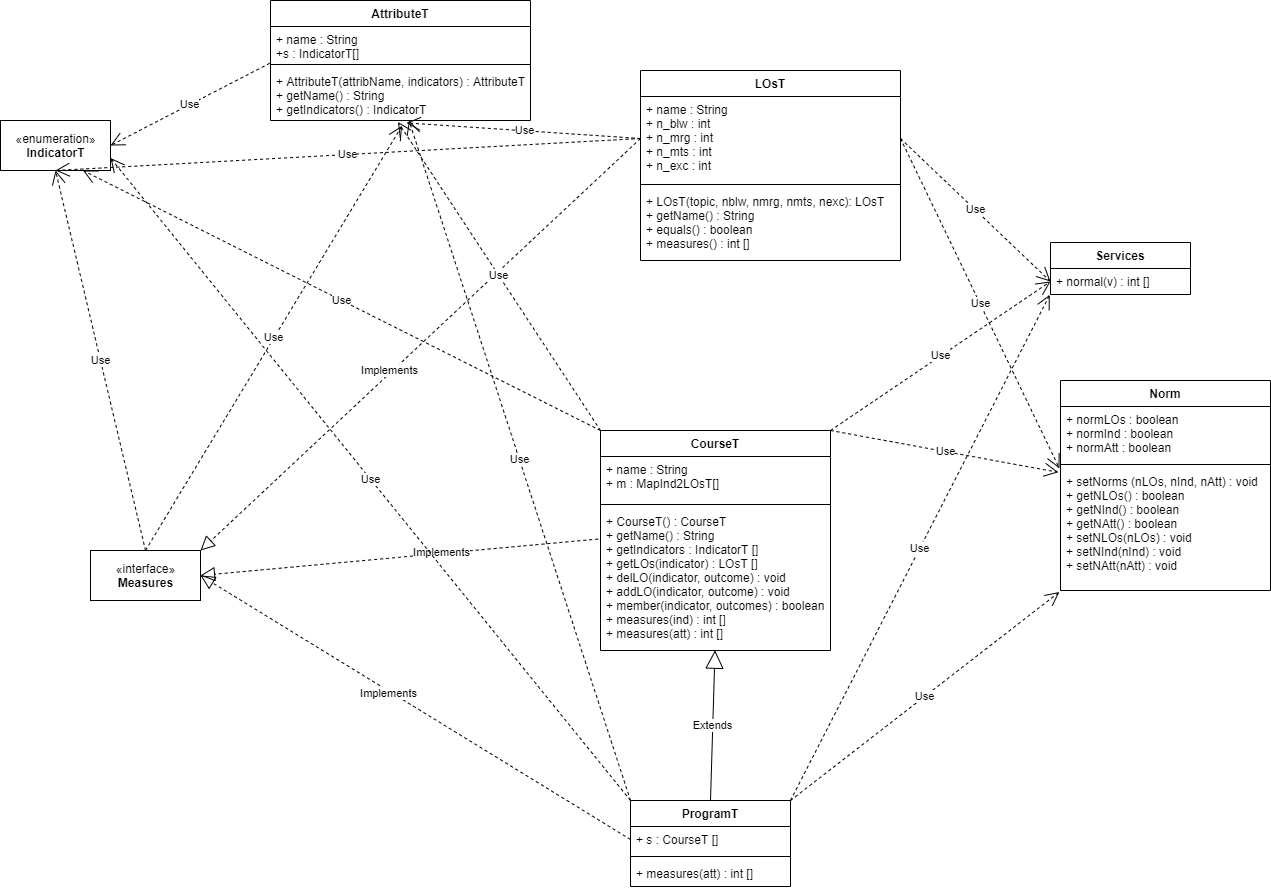
\includegraphics[scale=0.4]{UMLdiagram.png}

\newpage
\subsection*{Convex Hull Algorithm CFG}
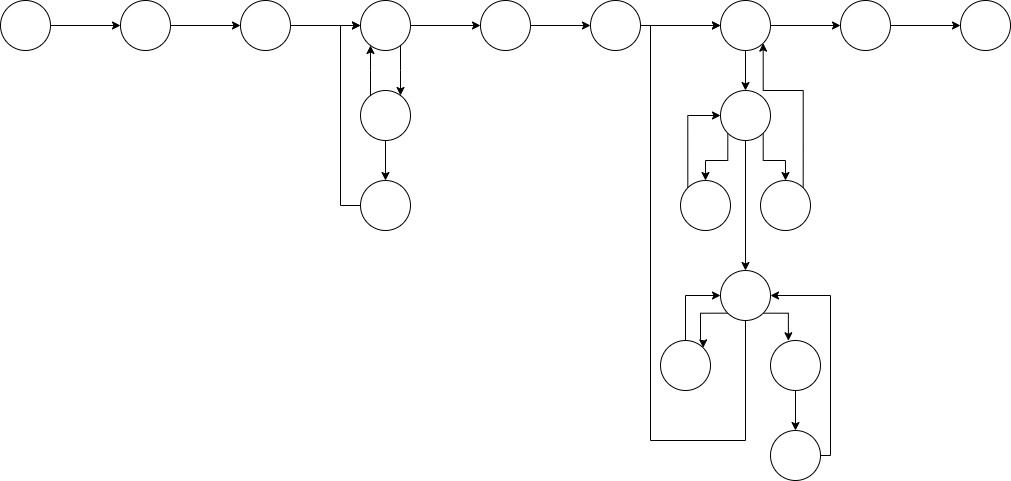
\includegraphics[scale=0.5]{CFG.png}

\end{document}
